\newgeometry{left=1.5in, right=1in, top=2in, bottom=1in}

\chapter{RESULTS AND DISCUSSION}

This chapter presents and discusses the results of fitted models that have been obtained from the study analysis.
Section \ref{sec:eda} presents the exploratory data analysis, section \ref{sec:model-diagnostics} presents the results of the fitted models, and section \ref{sec:model-results} presents model assumptions and diagnostics.


\section{Exploratory Data Analysis} \label{sec:eda}

\hspace*{0.5pt}
\addtocounter{table}{-1}

\begin{spacing}{0.8}
    \begin{small}
        \TableCaption{Summary of MCET Data} \label{tab:mcet-data-summary}
        \begin{longtable}{p{0.61in}p{0.5in}R{0.25in}R{0.35in}R{0.4in}R{0.31in}R{0.4in}R{0.2in}R{0.4in}R{0.3in}R{0.3in}}
            \toprule
            Variable  & Level   & n   & \%      & Missing & \%     & Mean   & SD   & Median & Min    & Max    \\
            \midrule
            TCCB ID   & -       & 543 & 98.9\%  & 6       & 1.1\%  & -      & -    & -      & -      & -      \\
            ePAL ID   & -       & 275 & 50.1\%  & 274     & 49.9\% & -      & -    & -      & -      & -      \\
            Sample ID & -       & 542 & 98.7\%  & 7       & 1.3\%  & -      & -    & -      & -      & -      \\
            Date      & -       & 540 & 98.4\%  & 9       & 1.6\%  & -      & -    & -      & -      & -      \\
            Latitude  & -       & 316 & 57.6\%  & 233     & 42.4\% & -15.79 & 0.04 & -15.78 & -15.87 & -15.70 \\
            Longitude & -       & 316 & 57.6\%  & 233     & 42.4\% & 35.04  & 0.03 & 35.03  & 34.97  & 35.10  \\
            Lineage   & -       & 255 & 46.4\%  & 294     & 53.6\% & -      & -    & -      & -      & -      \\
            & Clade 0 & 132 & 51.8\%* & -       & -      & -      & -    & -      & -      & -      \\
            & Clade 1 & 14  & 5.5\%*  & -       & -      & -      & -    & -      & -      & -      \\
            & Clade 2 & 47  & 18.4\%* & -       & -      & -      & -    & -      & -      & -      \\
            & Clade 3 & 14  & 5.5\%*  & -       & -      & -      & -    & -      & -      & -      \\
            & Clade 4 & 9   & 3.5\%*  & -       & -      & -      & -    & -      & -      & -      \\
            & Clade 5 & 15  & 5.9\%*  & -       & -      & -      & -    & -      & -      & -      \\
            & Clade 6 & 24  & 9.4\%*  & -       & -      & -      & -    & -      & -      & -      \\
            \bottomrule

        \end{longtable}
        * the percentages for the different clades are out of 255 and not 549 as for all the other percentages
    \end{small}
\end{spacing}


The final merged MCET dataset which has been used in this project have 549 

\restoregeometry

observations.
These observations are blood culture-confirmed typhoid fever cases of patients, under the age of 10 years, who resides in urban Blantyre.
Out of these, 316 cases have spatial information while 540 cases have temporal information.
310 cases have both spatial and temporal information and 255 of the 310 cases have genomic information.
Figure \ref{fig:flow-diagram} shows the merging process of the data tables.

Table \ref{tab:mcet-data-summary} summarises the variables in the merged data.
The variables used for the spatial and spatio-temporal analysis are \textit{Date} which is a date variable, and \textit{Latitude} and \textit{Longitude} which are latitude and longitude variables.
The variable \textit{Lineage} records genomic data.
The patients and sample ID variables (TCCB ID, ePAL ID and Sample ID) were used for merging the different data tables.

\begin{figure}[H]
    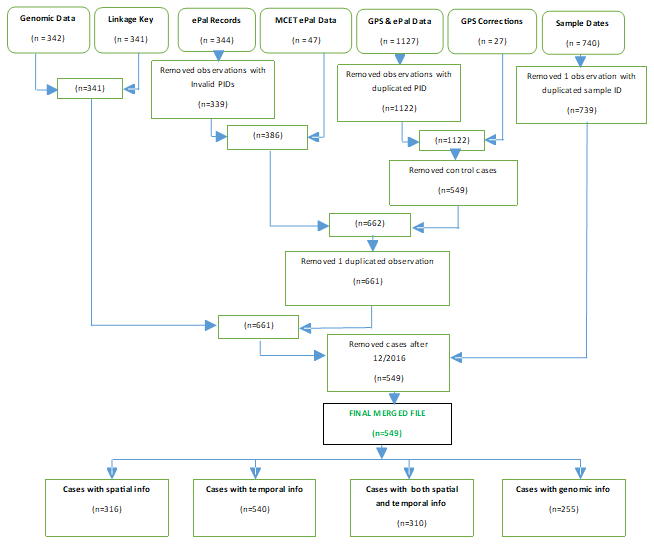
\includegraphics[scale=0.85]{MCET_Project_Data_Merging_Flow_Diagram.png}
    \FigureCaption {Flow diagram for the data merging process} \label{fig:flow-diagram}
\end{figure}

Figure \ref{fig:all-cumulative-cases} (Top) shows the cumulative frequency of the 540 cases with recorded temporal information during the study period.
The first case was recruited on 28th March 2015.
The last case was recruited on 30th December 2016.
Number of cases per day ranged from 1 to 6 cases.
The figure shows that there was a steady increase of typhoid fever cases across the study period.
Figure \ref{fig:all-cumulative-cases} (Bottom) shows the cumulative frequency of the 255 typhoid fever cases for which whole genome sequencing (WGS) was performed.
Clade 0 and 2 were recorded consistently throughout the study period.
Cases for clade 4 sub-lineage started appearing only from January 2016.

\begin{figure}[H]
    \begin{center}
        \includegraphics[scale=0.8]{Cumulative Cases Over Time (All Cases) and Cumulative Cases Over Time By Sub-Lineage.png}
    \end{center}
    \FigureCaption{Top: Cumulative cases over time for all 540 typhoid cases. Bottom: Cumulative cases of 255 typhoid cases with genomic data over time}
    \label{fig:all-cumulative-cases}
\end{figure}

\begin{figure}[H]
    \begin{center}
        \includegraphics[scale=0.8]{Sub-lineage.png}
    \end{center}
    \FigureCaption{Barplot of H58 Genomic Sub-Lineages for Salmonella typhi}
    \label{fig:salmonella-frequency-distribution}
\end{figure}

Figure \ref{fig:salmonella-frequency-distribution} shows the frequency distribution of the typhoid fever cases by sub-lineage.
The figure shows that clade 0 was the most common genomic sub-lineage representing 52\% of the reported cases followed by clade 2 at 18\%.
The other sub-lineages (clade 1, clade 3, clade 4, clade 5 and clade 6) had few cases, as such, they were grouped for modelling purposes.
In the proceeding sections, the grouped sub-lineages are being called \emph{grouped clades}.

\begin{figure}[H]
    \begin{center}
        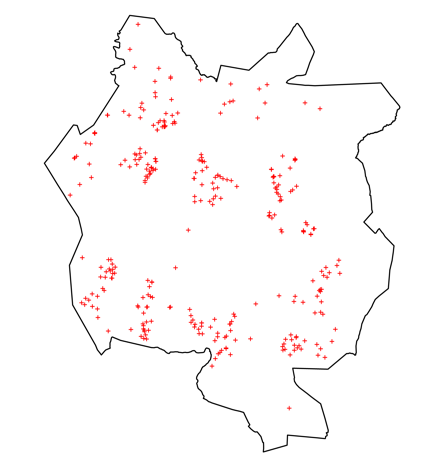
\includegraphics[scale=0.7]{Spatial distribution of typhoid fever in Blantyre city.png}
    \end{center}
    \FigureCaption{Spatial distribution of typhoid fever in Blantyre city} \label{fig:salmonella-spatial-distribution}
\end{figure}

Figure \ref{fig:salmonella-spatial-distribution} shows the spatial distribution of typhoid fever cases which were registered between March 2015 and December 2016 in Blantyre city.
The figure shows there was heterogeneous distribution of the cases with several clusters.
For example, it appears that there may be a cluster of cases in Ndirande, Bangwe, Nkolokoti-Kachere, Nancholi, Chilomoni, Chigumula, Mbayani-Chemusa and Chirimba.
The figure also shows that most of the cases appear to occur in peri-urban areas.


\begin{figure}[H]
    \begin{center}
        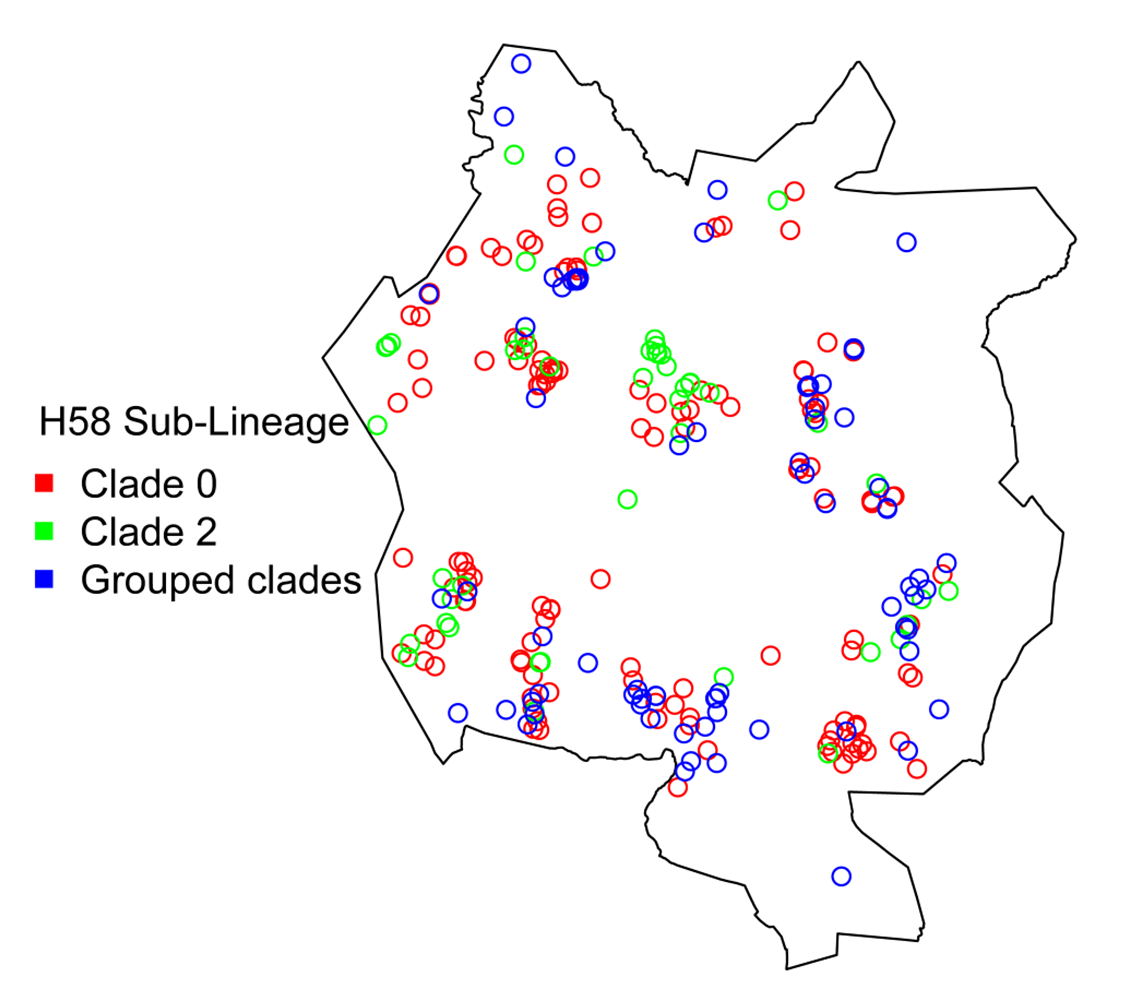
\includegraphics[scale=0.7]{Spatial distribution of typhoid fever in Blantyre by sub-lineage.png}
    \end{center}
    \FigureCaption{Spatial distribution of typhoid fever in Blantyre by sub-lineage} \label{fig:salmonella-genomic-sub-lineage}
\end{figure}

Out of the 549 typhoid cases in the final merged dataset, 255 cases had genomic data.
Figure \ref{fig:salmonella-genomic-sub-lineage} shows the spatial distribution of the 255 typhoid cases by genomic sub-lineage.
Out of the 7 sub-lineages, 5 of them caused relatively few typhoid cases during the study period.
These were grouped into one sub-lineage (grouped clades) during the modelling process.


\section{Model Diagnostics} \label{sec:model-diagnostics}

This section will discuss some of the techniques which were used to assess the validity of the fitted models for inference. 
The \textit{lgcp} package fits Bayesian spatial and spatio-temporal models. 
As such, the diagnostics presented in this section focus on assessing the MCMC iterations. 
All statistical analyses were conducted using R statistical software, version 4.0.3. 
The models were fitted using the \textit{lgcp} R package. 
These diagnostic techniques include log-target, trace plots and autocorrelation plots. 
Metropolis-adjusted Langevin algorithm
(MALA) length for all four spatio-temporal models was 1 million iterations.
Burn-in was 100,000 iterations.
Every 90th sample was retained.
For the multi-type spatial LGCP model, however, to achieve the desired convergence and minimise autocorrelation, the MALA length was 40 million iterations with 500,000 burn-in iterations and 18,000 as the thinning parameter.

\subsection{Log-Target}

\begin{figure}[H]
    \begin{center}
        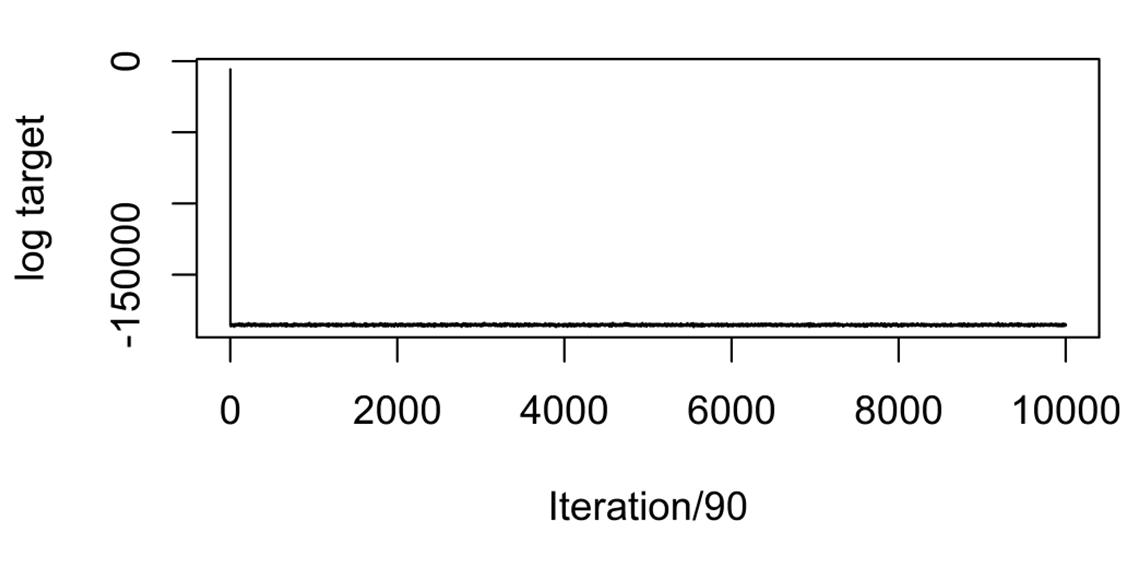
\includegraphics[scale=0.8]{Log Target Plot - ST - All Cases.png}
    \end{center}
    \FigureCaption{Plot of the log posterior over the duration of the MCMC run and burn-in for the spatio-temporal model for all cases} \label{fig:log-target-plot-for-all-cases}
\end{figure}

Log of the target posterior likelihood is used to check whether the Markov chain of the model being fitted is mixing well. 
The log target also checks convergence of the Markov chain to a posterior mode. 
The technique assesses the plot of $log\lbrace \pi\left( \beta, \eta, Y \mid X \right) \rbrace + c$ up to an additive constant $c$.

Figure \ref{fig:log-target-plot-for-all-cases} shows that the log-target of the Markov chain started with values near $0$ but quickly converged around $-200,000$. 
The convergence of the log of the target posterior likelihood means that the Markov chain is mixing well and the parameters of the fitted model can be used for inference.

\begin{figure}[H]
    \begin{center}
        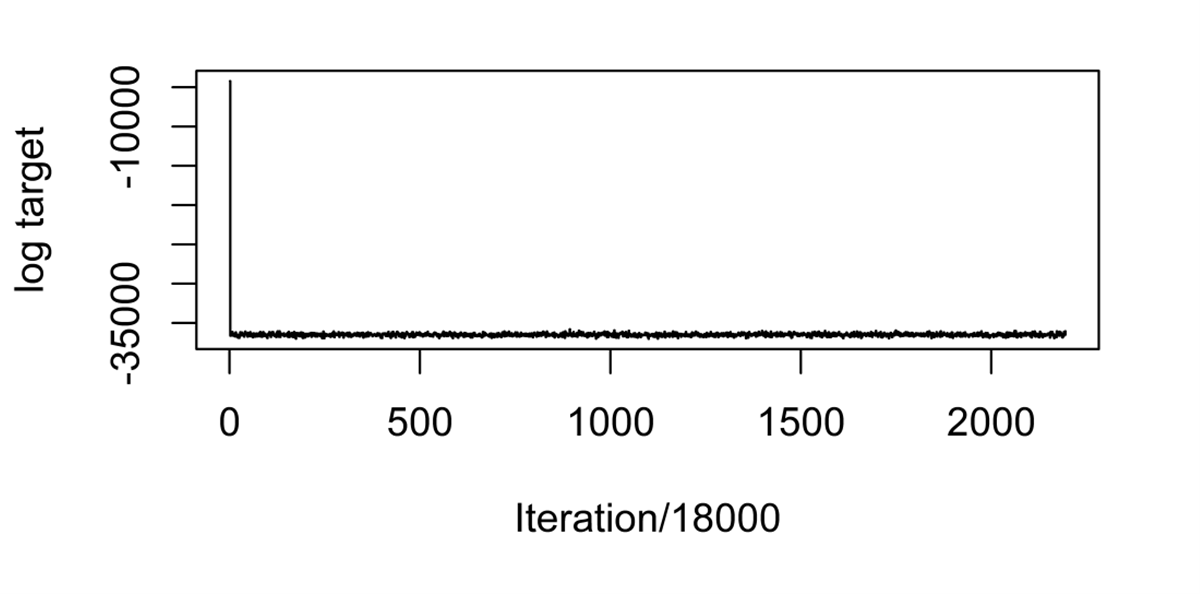
\includegraphics[scale=1]{Log Target - Multi-type.png}
    \end{center}
    \FigureCaption{Plot of the log posterior over the duration of the MCMC run and burn-in the multi-type spatial model} \label{fig:log-target-plot-multi-type}
\end{figure}

Figure \ref{fig:log-target-plot-multi-type} also shows that the log-target of the Markov chain of the multi-type spatial model converged at around $-35000$. The other three spatio-temporal models have similar convergence of their log-targets. For more details, see Appendix 1.

\subsection{Trace Plots}

Another intuitive and easily implemented diagnostic tool is a trace plot
which plots the parameter value of the model at time $t$ against the iteration
number. If the MCMC has converged to a stationary distribution, the trace plot will fluctuate randomly around the mode of the distribution. The trace plot looks like a hairy caterpillar when the posterior has converged to the stationary distribution. On the other hand, non-convergence can take many shapes. The two most common would be: 1. Clear trend in parameter values over iteration number 2. Switching back and forth between different parameter sets.

Figure \ref{fig:trace-plots-all-cases} and Figure \ref{fig:trace-plots-multi-type} show no obvious signs of non-convergence and are consistent with an MCMC process that converged successfully. The trace plots of the other three spatio-temporal models also show no obvious signs of non-convergence. See Appendix 2 for details.

\begin{figure}[H]
    \begin{center}
        \includegraphics[scale=1]{Traceplots for Beta and Eta - All Cases.png}
    \end{center}
    \FigureCaption{Traceplots of the model parameters of the spatio-temporal model with all cases} \label{fig:trace-plots-all-cases}
\end{figure}

\begin{figure}[H]
    \begin{center}
        \includegraphics[scale=1]{Traceplot - Multi-type.png}
    \end{center}
    \FigureCaption{Traceplots of the model parameters of the multi-type spatial model} \label{fig:trace-plots-multi-type}
\end{figure}

\subsection{Autocorrelation in the Latent Gaussian Field}

Spatial autocorrelation is the association of a variable with itself through space. When the values in adjacent spatial region vary together in opposite directions, negative autocorrelation occurs. Whereas when similar values occur near one another, positive autocorrelation occurs.

Figures in Appendix 3 show autocorrelation of MCMC iterations for each cell on the computational grid. Initially, there are positive autocorrelation at cellwise lag of 1 but little to no autocorrelation at cellwise lag of 15 for both spatio-temporal model with all cases and multi-type spatial model. This shows that there is very little autocorrelation in the sampled values of the retained latent field. Computational grid cell width is 350 metres. The other three spatio-temporal models also produced similar autocorrelation results. See Appendix 3 for details. Computational grid cell width is 350 metres.

\subsection{Autocorrelation of Parameters from the Point Process}

Figure \ref{fig:correlation-plots-all-cases} shows that some parameters, $\phi$ and $\theta$ in the spatio-temporal model exhibit substantial autocorrelation, so the MALA algorithm will be slow to explore the entire posterior distribution. This can be resolved by increasing the posterior sample of the model by running the MALA algorithm longer. Since the autocorrelation is not severe at lag 40 of the thinned iterations of the MCMC for $\theta$ and the rest of the parameters show no autocorrelation, there is no need to run the MCMC longer. The other spatio-temporal models also show similar results. See Appendix 4 for details. Figure \ref{fig:correlation-plots-multi-type}, on the other hand, shows little autocorrelation for the multi-type spatial model at different lags in the thinned samples.

\begin{figure}[h]
    \begin{center}
        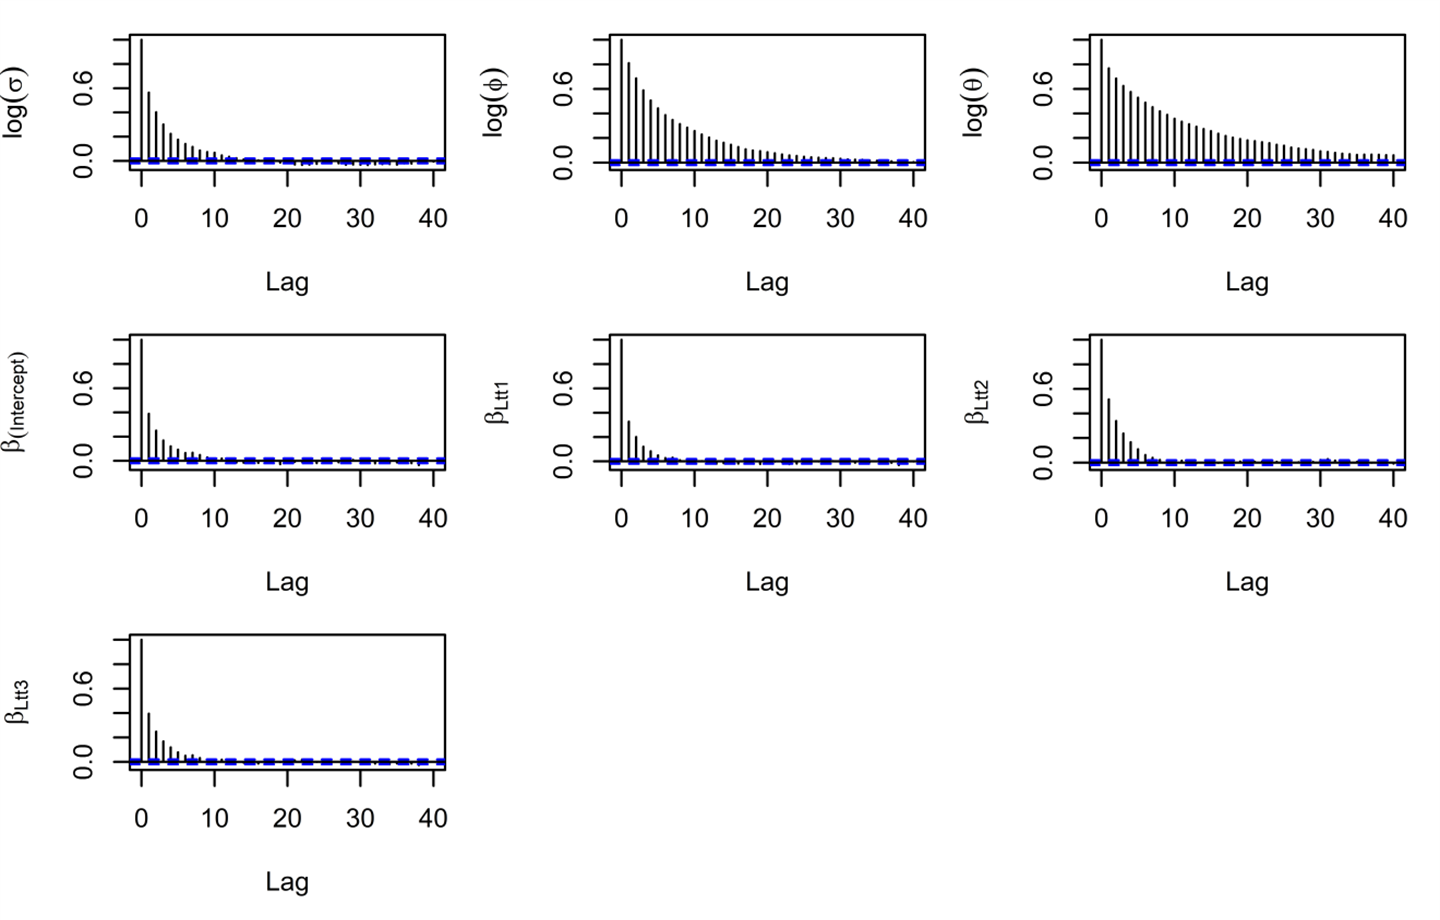
\includegraphics[scale=1]{Autocorrelation of Beta and Eta - All Cases.png}
    \end{center}
    \FigureCaption{Autocorrelation plots of the parameters of the Gaussian latent field from the spatio-temporal model with all cases} \label{fig:correlation-plots-all-cases}
\end{figure}

\begin{figure}[H]
    \begin{center}
        \includegraphics[scale=1]{Autocorrelation of Beta and Eta - Multi-type.png}
    \end{center}
    \FigureCaption{Autocorrelation plots of the parameters of the Gaussian latent field for multi-type spatial model} \label{fig:correlation-plots-multi-type}
\end{figure}


\section{Log-Gaussian Cox Process Results} \label{sec:model-results}

This section will discuss the results of the four spatio-temporal models and the multi-type spatial model which have been fitted using the LGCP framework. 
All models used a computational grid of cells 350 x 350 metres in dimension.

\subsection{Spatio-Temporal Model with All Cases}

This subsection discusses the results of the spatio-temporal model fitted using all typhoid fever cases without focusing on their genomic lineage. 
In this paper, the covariance function of the Gaussian process used an exponential model. 
Table \ref{tab:lgcp-model-all-cases} summarises the parameters of the latent field of the spatio-temporal LGCP model with all typhoid cases. 
The standard deviation parameter $\sigma$ had median 2.185 (95\% CrI 1.93 to 2.497); the spatial correlation parameter $\phi$ had median 940.1 metres (95\% CrI 709 to 1275); and the temporal correlation parameter $\theta$ had median 0.075 months (95\% CrI 0.050 to 0.107). 
This means that spatial dependence had a median of about 940 metres and a temporal dependence had a median of about 2 days. 
The other parameters, $t^{'}, t^{''}$ and $t^{'''}$ are for the cubic B-spline which was included to assess the temporal distribution of the model and has not been interpreted to have a covariate effects. The prior and posterior plot in Appendix 8 shows that $\sigma$ has relatively a wider departure from the prior compared with the parameter $\phi$. Therefore statistical inference must be done cautiously.

\hspace*{0.2pt}
\addtocounter{table}{-1}

\begin{spacing}{0.85}
    \TableCaption{Parameter estimates for the LGCP model with all cases}  \label{tab:lgcp-model-all-cases}
    \begin{longtable}{p{1.3in}p{1.3in}p{1.3in}p{1.3in}}
        \toprule
        Parameter                & Median               & Lower 95\%  CrI        & Upper 95\%  CrI        \\ \midrule
        $\sigma$                 & 2.185                & 1.93                 & 2.497                \\
        $\phi$                   & 940.1                & 709                  & 1275                 \\
        $\theta$                 & 7.46$\times10^{-2}$  & 4.952$\times10^{-2}$ & 0.1072               \\
        $exp(\beta_{Intercept})$ & 8.912$\times10^{-9}$ & 3.038$\times10^{-9}$ & 2.462$\times10^{-8}$ \\
        $exp(\beta_{t^{'}})$     & 59.81                & 7.31                 & 649.9                \\
        $exp(\beta_{t^{''}})$    & 2.146                & 0.4726               & 9.768                \\
        $exp(\beta_{t^{'''}})$   & 4.144                & 1.16                 & 15.98                \\
        \bottomrule
    \end{longtable}
\end{spacing}


\begin{figure}[H]
    \begin{center}
        \includegraphics[scale=0.8]{Posterior Covariance Function - All Cases.png}
    \end{center}
    \FigureCaption{Plots of the posterior spatial covariance (Left) and temporal correlation (Right) for the Gaussian process of the spatio-temporal model with all cases} \label{fig:covariance-function-all-cases}
\end{figure}

To assess the posterior dependence between cells on the computational grid,   exponential model for the posterior covariance function of the Gaussian process was used. Figure \ref{fig:covariance-function-all-cases} shows the shape of the posterior covariance function for the spatio-temporal model with all cases. The figure shows that the posterior dependence between cells is over a small range in both time and space. Figure \ref{fig:k-function-all-cases}, the inhomogeneous K function plot, shows that the points formed clusters at about 2.5km radius for all correction estimates (isotropic correction estimates, translation correction estimates, modified border correction estimates and border corrected estimates).

\begin{figure}[H]
    \begin{center}
        \includegraphics[scale=0.75]{Inhomogeneous K Function - All Cases.png}
    \end{center}
    \FigureCaption{Inhomogeneous K Function for all typhoid cases} \label{fig:k-function-all-cases}
\end{figure}

\begin{figure}[H]
    \begin{center}
        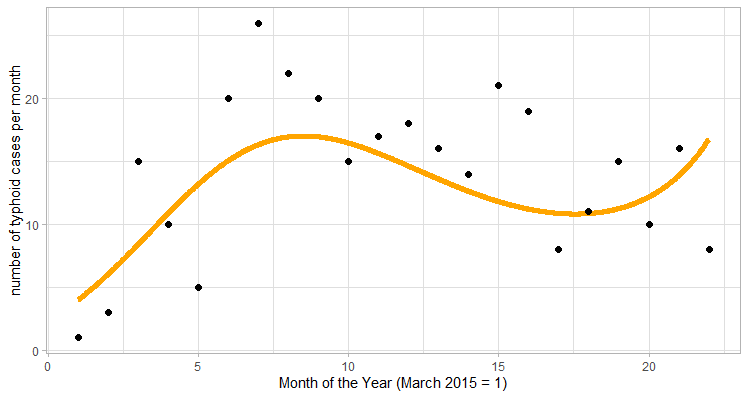
\includegraphics[scale=0.75]{Long term trend of temporal model - All Cases.png}
    \end{center}
    \FigureCaption{Temporal distribution of typhoid fever outbreak for all typhoid cases} \label{fig:temporal-distribution-all-cases}
\end{figure}

To ascertain the temporal distribution of the typhoid fever outbreak, a cubic B-spline was used. The orange graph line of Figure \ref{fig:temporal-distribution-all-cases} describes the trend of the typhoid fever between March 2015 to December 2016 that was fitted using B-splines. The figure shows that the typhoid fever outbreak was at the peak around the months of October and November 2015. Then the cases started decreasing steadily up to July 2016 when it started increasing steadily again.

\begin{figure}[h]
    \begin{center}
        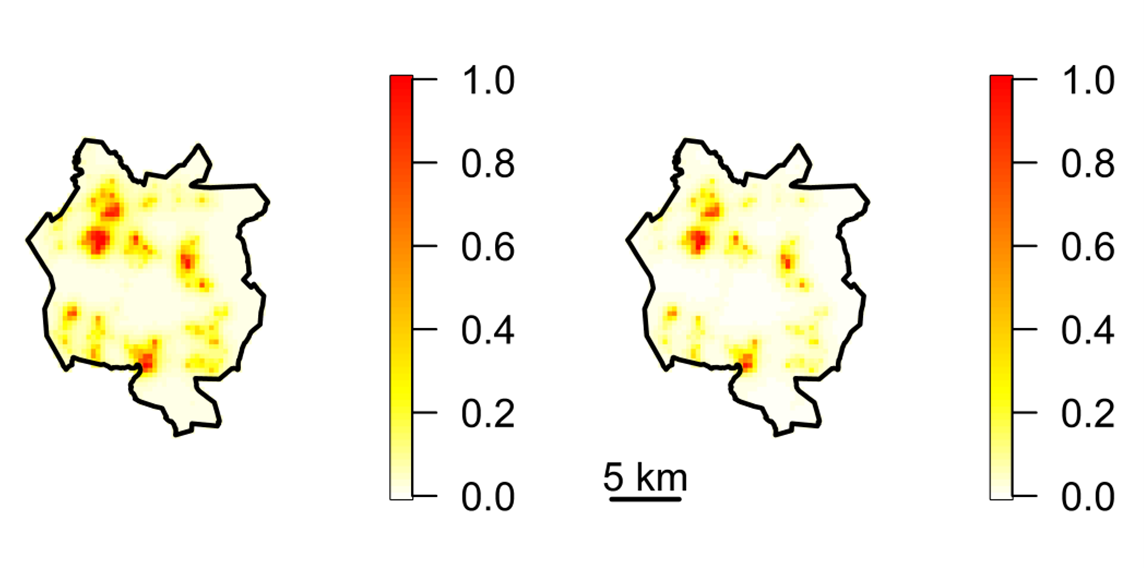
\includegraphics[scale=1.2]{Exceedance Probabilities - All Cases.png}
    \end{center}
    \FigureCaption{Exceedance plot of posterior probability that the incidence rates exceed 2 (left) and 4 (right) for all typhoid cases} \label{fig:exceedance-plot-all-cases}
\end{figure}

Figure \ref{fig:exceedance-plot-all-cases} shows location of high posterior probability that incidence rate for all typhoid fever cases exceeds 2 and 4. The figure shows that Chilobwe-Misesa, Mbayani-Chemusa, Chirimba, Nkolokoti-Kachere, Nancholi-Manase, Ndirande and Bangwe-Namiyango were the hotspots of typhoid fever during the outbreak. These areas had a high posterior probability to have a 4 times higher incidence rate of typhoid than the rest of Blantyre city.

\subsection{Spatio-Temporal Model for Clade 0 Sub-Lineage}

This sub-section discusses the findings of spatio-temporal model for clade 0 sub-lineage of H58 lineage of \textit{S. typhi}.

\newpage

\addtocounter{table}{-1}
\begin{spacing}{0.9}
    \TableCaption{Parameter estimates for the LGCP model for clade 0 cases} \label{tab:lgcp-model-zero-cases}
    \begin{longtable}{p{1.3in}p{1.3in}p{1.3in}p{1.3in}}
        \toprule
        Parameter                & Median              & Lower 95\% CrI       & Upper 95\% CrI       \\ \midrule
        $\sigma$                 & 2.257               & 1.893                & 2.683                \\
        $\phi$                   & 873.6               & 615                  & 1316                 \\
        $\theta$                 & 0.1068              & 6.417$\times10^{-2}$ & 0.1747               \\
        $exp(\beta_{Intercept})$ & 1.28$\times10^{-8}$ & 4.223$\times10^{-9}$ & 3.663$\times10^{-8}$ \\
        $exp(\beta_{t^{'}})$     & 3.634               & 0.3014               & 52.46                \\
        $exp(\beta_{t^{''}})$    & 2.912               & 0.4509               & 20.95                \\
        $exp(\beta_{t^{'''}})$   & 1.443               & 0.3212               & 6.102                \\
        \bottomrule
    \end{longtable}
\end{spacing}

\hspace*{0.2pt}

Table \ref{tab:lgcp-model-zero-cases} summarises the estimated parameters of the Gaussian process whose realisation produced typhoid cases which were caused by clade 0. The standard deviation parameter $\sigma$ had median 2.257 (95\% CrI 1.893 to 2.683); the spatial correlation parameter $\phi$ had median 873.6 metres (95\% CrI 615 to 1316); and the temporal correlation parameter $\theta$ had median 0.107 months (95\% CrI 0.064 to 0.175). This means that clade 0 cases had spatial dependence had a median of about 874 metres and a temporal dependence had a median of about 3 days.

\begin{figure}[H]
    \begin{center}
        \includegraphics[scale=0.8]{Posterior Covariance Function - Major 0.png}
    \end{center}
    \FigureCaption{Plots of the posterior spatial covariance (Left) and temporal correlation (Right) for the Gaussian process of the spatio-temporal model for clade 0 cases} \label{fig:spatio-temporal-model-zero-cases}
\end{figure}

\begin{figure}[H]
    \begin{center}
        \includegraphics[scale=1]{Inhomogeneous K Function - Major 0.png}
    \end{center}
    \FigureCaption{Inhomogeneous K Function for clade 0 cases} \label{fig:k-function-zero-cases}
\end{figure}

Figure \ref{fig:spatio-temporal-model-zero-cases} shows the posterior covariance function for the Gaussian process of spatio-temporal model for clade 0 cases. The figure confirms the results above as it shows that the posterior dependence between cells is over a small range in both time and space. Figure \ref{fig:k-function-zero-cases}, the inhomogeneous K function plot also, shows that the points formed clusters at about 1.5km radius for all correction estimates (isotropic correction estimates, translation correction estimates, modified border correction estimates and border corrected estimates).

The orange graph line of Figure \ref{fig:temporal-distribution-zero-cases}, fitted using the coefficients of $t^{'}, t^{''}$ and $t^{'''}$, the B-spline basis functions, shows that cases of typhoid fever from clade 0 sub-lineage started increasing since its first registration in April 2015 and reached its first peak in October 2015. The cases started decreasing from December 2015 until they started increasing again from May 2016 up to the end of the study. Clade 0 cases were registered between April 2015 to October 2016. The temporal trend of clade 0 is similar to that of all cases.

\begin{figure}[H]
    \begin{center}
        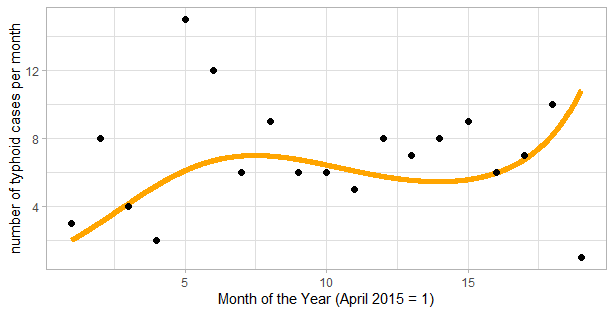
\includegraphics[scale=0.9]{Long term trend of temporal model - Major 0.png}
    \end{center}
    \FigureCaption{Temporal distribution of typhoid fever outbreak for clade 0 cases} \label{fig:temporal-distribution-zero-cases}
\end{figure}

Comparing the parameters of the two models, it is clear that the point estimates of $\sigma$ for the two models were similar. For spatio-temporal model with all cases, $\sigma$ was 2.185 (95\% CrI 1.93 to 2.497) while for clade 0 was 2.257 (95\% CrI 1.893 to 2.683). The point estimates of $\phi$ from the two models were different. For all cases, the median was 940.1 metres (95\% CrI 709 to 1275) while for clade 0 cases the median was 873.6 metres (95\% CrI 615 to 1316). The difference can also be explained by the inhomogeneous K function plots which show that typhoid fever for all cases and for clade 0 cases formed cluster at 2.5km radius and 1.5km radius respectively. This means that the cases for clade 0 cluster tightly than for all cases. This means that the typhoid fever cases caused by clade 0 had more local transmission of typhoid fever. The point estimates for $\theta$, the parameter which scales the temporal dependence, were also different for the two models with all cases registering 0.075 months  (95\% CrI 0.050 to 0.107) while clade 0 registering 0.107 months (95\% CrI 0.064 to 0.175). This means that all cases happened at shorter intervals of 2 days compared to 3 days for clade 0 cases. The wider credible intervals for all point estimates for clade 0 give evidence of uncertainty in the estimates. This is because the number of typhoid fever cases caused by clade 0 were only 43\% of all typhoid fever cases.

Figure \ref{fig:exceedance-plot-zero-cases} shows location of high posterior probability that incidence rates exceeds 2 and 4 for all typhoid fever cases caused by clade 0 sub-lineage of the H58 lineage of \textit{S. typhi}. The figure shows that Mbayani-Chemusa, Chirimba, Nkolokoti-Kachere, Nancholi-Manase and Ndirande had 4 times higher incidence rate of typhoid fever outbreak caused by clade 0 sub-lineage of H58 lineage of \textit{S. typhi} than other locations in the city. These locations are five of the seven locations with 4 times higher incidence rates of typhoid fever for all cases. The spatial distribution for clade 0 is similar to the spatial distribution for all cases of typhoid fever. One of the reasons could be because clade 0 sub-lineage of H58 haplotype of \textit{S. typhi} was the main cause of typhoid fever cases in the recent typhoid fever outbreak. It caused 52\% of all the registered typhoid cases with genomic data.

\begin{figure}[H]
    \begin{center}
        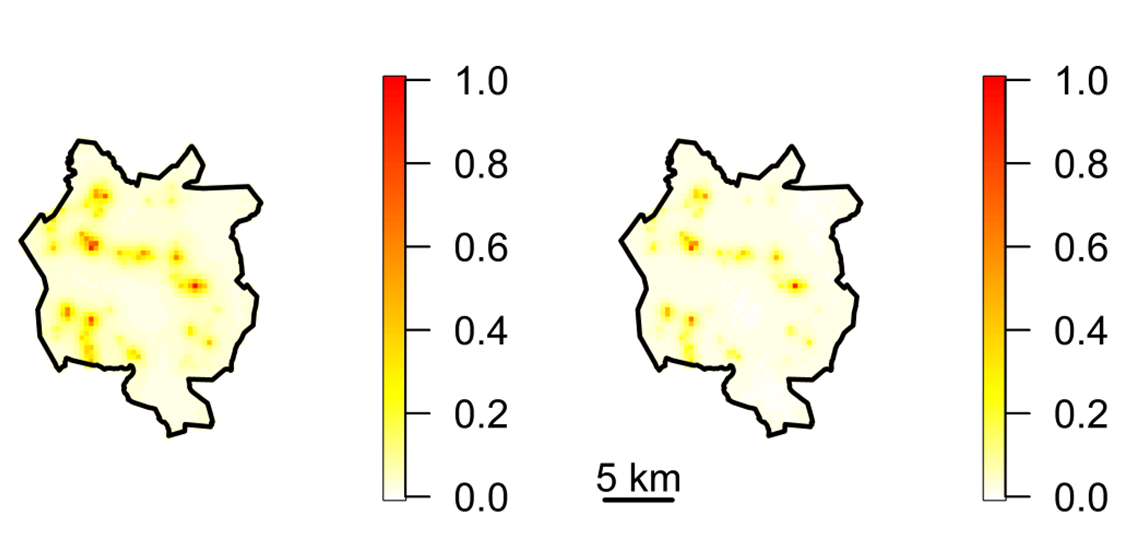
\includegraphics[scale=0.8]{Exceedance Probabilities - Major 0.png}
    \end{center}
    \FigureCaption{Exceedance Plot of posterior probability that the incidence rate exceeds 2 (left) and 4 (right) for clade 0 cases} \label{fig:exceedance-plot-zero-cases}
\end{figure}

\subsection{Spatio-Temporal Model for Clade 2 Sub-Lineage}

This sub-section discusses the findings of spatio-temporal model for clade 2 sub-lineage of H58 lineage of \textit{S. typhi}.

\hspace*{0.2pt}
\addtocounter{table}{-1}
\begin{spacing}{0.9}
    \TableCaption{Parameter estimates for the LGCP model for clade 2 cases}  \label{tab:lgcp-model-two-cases}
    \begin{longtable}{p{1.3in}p{1.3in}p{1.3in}p{1.3in}}

        \toprule
        Parameter               & Median               & Lower 95\% CrI        & Upper 95\% CrI       \\ \midrule
        $\sigma$                & 2.483                & 1.884                 & 3.243                \\
        $\phi$                  & 807                  & 501.7                 & 1360                 \\
        $\theta$                & 0.3261               & 0.1707                & 0.6065               \\
        $exp(beta_{Intercept})$ & 3.961$\times10^{-8}$ & 1.074$\times10^{-10}$ & 1.295$\times10^{-5}$ \\
        $exp(\beta_{t^{'}})$    & 0.2223               & 1.283$\times10^{-6}$  & 44367                \\
        $exp(\beta_{t^{''}})$   & 0.3273               & 4.556$\times10^{-3}$  & 24.61                \\
        $exp(\beta_{t^{'''}})$  & 0.2341               & 3.564$\times10^{-4}$  & 159.8                \\
        \bottomrule

    \end{longtable}
\end{spacing}

\hspace*{2pt}

\begin{figure}[H]
    \begin{center}
        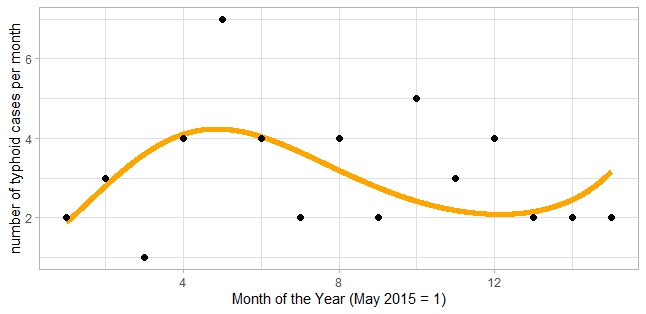
\includegraphics[scale=0.85]{Long term trend of temporal model - Major 2.png}
    \end{center}
    \FigureCaption{Temporal distribution of typhoid fever outbreak for clade 2 cases} \label{fig:temporal-distribution-two-cases}
\end{figure}

Table \ref{tab:lgcp-model-two-cases} is the summary of the parameters of the latent field of the spatio-temporal LGCP model with clade 2 typhoid cases. The parameter $\sigma$ had median 2.483 (95\% CrI 1.884 to 3.243); the parameter $\phi$ had median 807 metres (95\% CrI 501.7 to 1360); and the parameter $\theta$ had median 0.326 months (95\% CrI 0.171 to 0.607). This means that the clade 2 cases had spatial dependence of about 807 metres and a temporal dependence of about 10 days. The orange graph line in Figure \ref{fig:temporal-distribution-two-cases} shows that cases of typhoid fever caused by clade 2 sub-lineage was highest in September 2015 and has been decreasing steadily during the study period. The temporal trend of clade 2 is similar to that of clade 0 and all cases discussed in the previous sections.

The posterior covariance function plot for the Gaussian process of spatio-temporal model for clade 2 cases in Appendix 5 shows that the posterior dependence between cells is over a small range in both time and space. The inhomogeneous K function plot in Appendix 9 shows that the points formed clusters at about 2.5km radius for all correction estimates (isotropic correction estimates, translation correction estimates, modified border correction estimates and border corrected estimates).

The comparison of parameters in Table \ref{tab:lgcp-model-two-cases} with those in Table \ref{tab:lgcp-model-zero-cases} and Table \ref{tab:lgcp-model-all-cases} show that $\sigma$ values from all the three models are similar. Their medians range from 2.185 to 2.483. The point estimate of $\phi$ for the model with clade 2 cases and all cases were different. Clade 2 has $\phi$ of median of 807 metres (95\% CrI 501.7 to 1360) while all cases has a median of 940.1 metres (95\% CrI 709 to 1275). $\phi$ for clade 2 is similar to the model with clade 0 cases with a 873.6 metres (95\% CrI 615 to 1316). All models have spatial dependence of less that 1km. The point estimate for $\theta$ from clade 0 and clade 2 were different. Clade 0 has a temporal dependence of 3 days while clade 2 has a temporal dependence of 10 days. The wider credible intervals for all point estimates for the model with clade 2 cases is due to the relatively fewer number of typhoid fever cases cause by clade 2 sub-lineage.

\begin{figure}[H]
    \begin{center}
        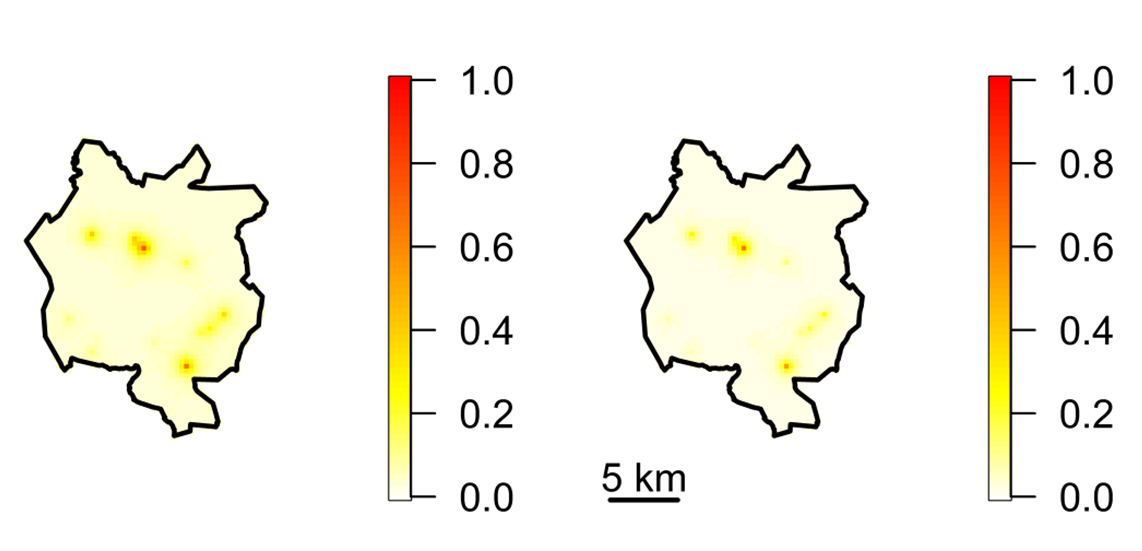
\includegraphics[scale=1]{Exceedance Probabilities - Major 2.png}
    \end{center}
    \FigureCaption{Exceedance Plot of posterior probability that the incidence rate exceeds 2 (left) and 4 (right) for clade 2 cases} \label{fig:exceedance-plot-two-cases}
\end{figure}

Figure \ref{fig:exceedance-plot-two-cases} shows location of high posterior probability that incidence rate of typhoid fever cases caused by clade 2 sub-lineage of the H58 lineage of \textit{S. typhi} exceeds 2 and 4. The figure shows that Ndirande and Chigumula had 4 times higher incidence rate of the typhoid fever outbreak than other locations in the city.

\subsection{Spatio-Temporal Model for Grouped Sub-Lineages}

This sub-section discusses the findings of spatio-temporal model for the genomic clades which had fewer typhoid cases (clade 1, clade 3, clade 4, clade 5 and clade 6). These were grouped into a single clade for model fitting.

\newpage

\hspace{0.5pt}

\addtocounter{table}{-1}
\begin{spacing}{0.9}
    \TableCaption{Parameter estimates for the LGCP model for grouped clades} \label{tab:lgcp-model-grouped-clades}
    \begin{longtable}{p{1.3in}p{1.3in}p{1.3in}p{1.3in}}
        \toprule
        Parameter               & Median               & Lower 95\% CrI        & Upper 95\% CrI       \\ \midrule
        $\sigma$                & 2.31                 & 1.858                 & 2.848                \\
        $\phi$                  & 791.7                & 495.7                 & 1264                 \\
        $\theta$                & 0.1785               & 0.1001                & 0.3175               \\
        $exp(beta_{Intercept})$ & 3.212$\times10^{-9}$ & 5.664$\times10^{-10}$ & 1.323$\times10^{-8}$ \\
        $exp(\beta_{t^{'}})$    & 27.04                & 0.7734                & 1569                 \\
        $exp(\beta_{t^{''}})$   & 7.471                & 0.7305                & 86.59                \\
        $exp(\beta_{t^{'''}})$  & 3.405                & 0.444                 & 31.2                 \\
        \bottomrule
    \end{longtable}
\end{spacing}

\hspace{0.2pt}

Table \ref{tab:lgcp-model-grouped-clades} is the summary of the parameters of the latent field of the spatio-temporal LGCP model with grouped clades. The parameter $\sigma$ had median 2.31 (95\% CrI 1.858 to 2.848); the parameter $\phi$ had median 791.7 metres (95\% CrI 495.7 to 1264); and the parameter $\theta$ had median 0.179 months (95\% CrI 0.100 to 0.318). The point estimate for the standard deviation parameter $\sigma$ for the grouped clades is similar to that of the other models. The spatial correlation parameter estimate $\phi$ for the grouped clades is also comparable with the other three models but the temporal correlation estimate $\theta$ is different from the rest of the models. But the credible intervals of the point estimates of the model with grouped cases is narrower than that of the model with clade 2 cases. This is because of the number of cases involved during modelling. Clade 2 has the lowest number of cases compared to the other models. See Table \ref{tab:lgcp-model-all-cases}, Table \ref{tab:lgcp-model-zero-cases}, Table \ref{tab:lgcp-model-two-cases} and Table \ref{tab:lgcp-model-grouped-clades} for details.

The orange graph line in Figure \ref{fig:temporal-distribution-grouped-clades} shows that cases of typhoid fever caused by the grouped clades had a steady increase after first registration in March 2015. The typhoid cases for the grouped sub-lineages were highest between October and November 2015. The cases started decreasing steadily from December 2015 until the end of the study. The temporal trend is relatively different from the temporal trend for all cases, clade 0 and clade 2. The temporal trend for models for all cases, clade 0 and clade 2 started increasing then decreasing and increasing again. The temporal trend for the grouped clades just increased and decreased steadily and flattened at the end without increasing again.

\begin{figure}[H]
    \begin{center}
        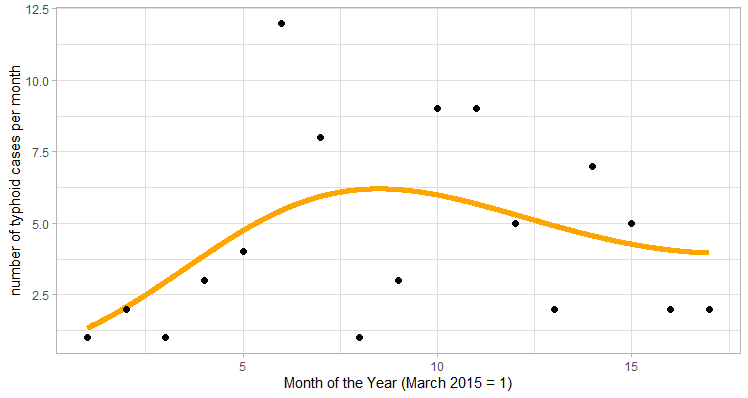
\includegraphics[scale=0.7]{Long term trend of temporal model - Major 13456.png}
    \end{center}
    \FigureCaption{Temporal distribution of typhoid fever outbreak for the grouped clades} \label{fig:temporal-distribution-grouped-clades}
\end{figure}

Figure \ref{fig:temporal-distribution-grouped-clades} is showing the location of high posterior probability that incidence rate of typhoid fever cases caused by the grouped clades of the H58 lineage of \textit{S. typhi} exceeds 2 and 4. The figure shows that Mbayani-Chemusa, Nkolokoti-Kachere, Bangwe-Namiyango, Nancholi-Manase and Chilobwe-Misesa had 4 times higher incidence rate of the typhoid fever outbreak than other locations in the city. The inhomogeneous K function plot in Appendix 9 shows evidence of clustering at the radius of about 2km for all correction estimates (isotropic correction estimates, translation correction estimates, modified border correction estimates and border corrected estimates).

\begin{figure}[H]
    \begin{center}
        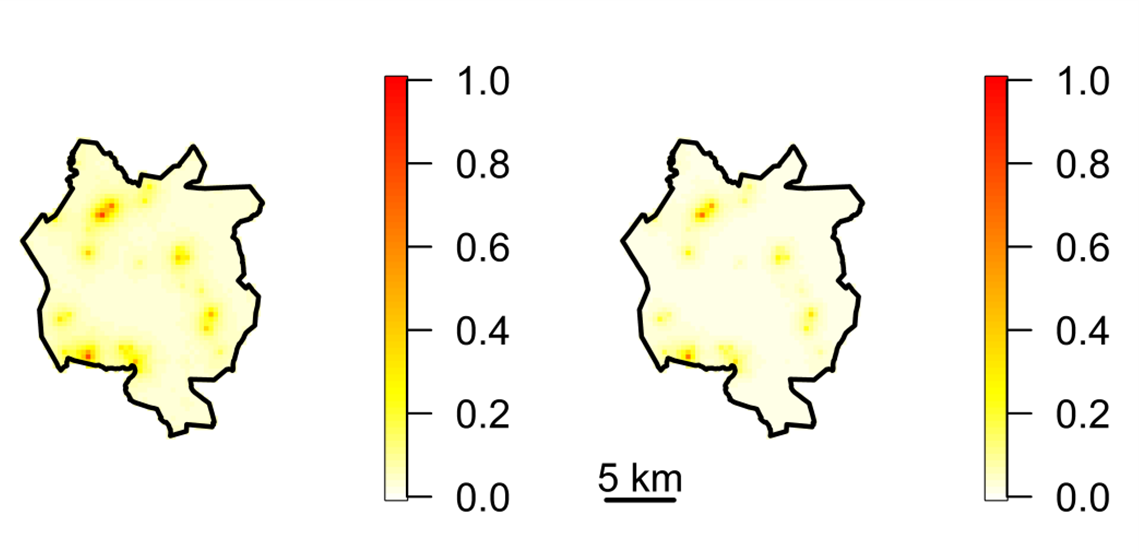
\includegraphics[scale=0.8]{Exceedance Probabilities - Major 13456.png}
    \end{center}
    \FigureCaption{Exceedance Plot of posterior probability that the incidence rate exceeds 2 (left) and 4 (right) for the grouped clades}\label{fig:exceedance-plot-posterior-probability}
\end{figure}

Mbayani-Chemusa is the only location in Blantyre which had high incidence rate of typhoid fever caused by all the three sub-lineages (clade 0, clade 2 and clade13456). This means that the spatial interaction of the sub-lineages were complementary. Ndirande had high incidence rate of typhoid fever caused by both clade 0 and clade 2 sub-lineages. The two sub-lineages were also complementary in space in this location. Bangwe-Namiyango had high incidence rate of typhoid fever caused by both clade 2 and the grouped clades while Nancholi-Manase and Nkolokoti-Kachere had high incidence rate of typhoid fever caused by both clade 0 and the grouped clades.

\subsection{Multi-Type Spatial Model}

This sub-section discusses the findings of the multi-type spatial model for the genomic clade 0, 2 and the other clades which had fewer cases and were combined into one clade.

Table \ref{tab:multivariate-spatial-model} is the summary of the estimated parameters of the Gaussian latent field of the multi-type spatial LGCP model for clade 0, clade 2 and the grouped clades. The parameter $\sigma_1$ had median 0.8735 (95\% CrI 0.4004 to 1.469); the parameter $\phi_1$ had median 1408 metres (95\% CrI 897.7 to 2190); the parameter $\sigma_2$ had median 1.293 (95\% CrI 0.6932 to 2.097); the parameter $\phi_2$ had median 1381 metres (95\% CrI 902.1 to 2142); the parameter $\sigma_3$ had median 1.158 (95\% CrI 0.6036 to 1.774); the parameter $\phi_3$ had median 1390 metres (95\% CrI 920.4 to 2153); the parameter $\sigma_4$ had median 2.091 (95\% CrI 1.674 to 2.678); the parameter $\phi_4$ had median 1192 metres (95\% CrI 895.6 to 1645).


\begin{spacing}{0.8}
    \TableCaption{Table of the parameter estimates from the multivariate spatial model} \label{tab:multivariate-spatial-model}
    \begin{longtable}{p{1.3in}p{1.3in}p{1.3in}p{1.3in}}
        \toprule
        Parameter                 & Median               & Lower 95\% CrI       & Upper 95\% CrI       \\ \midrule
        $\sigma_1$                & 0.8735               & 0.4004               & 1.469                \\
        $\phi_1$                  & 1408                 & 897.7                & 2190                 \\
        $\sigma_2$                & 1.293                & 0.6932               & 2.097                \\
        $\phi_2$                  & 1381                 & 902.1                & 2142                 \\
        $\sigma_3$                & 1.158                & 0.6036               & 1.774                \\
        $\phi_3$                  & 1390                 & 920.4                & 2153                 \\
        $\sigma_4$                & 2.091                & 1.674                & 2.678                \\
        $\phi_4$                  & 1192                 & 895.6                & 1645                 \\
        $exp[\beta_1(Intercept)]$ & 5.572$\times10^{-7}$ & 2.266$\times10^{-7}$ & 2.097$\times10^{-6}$ \\
        $exp[\beta_2(Intercept)]$ & 2.118$\times10^{-7}$ & 7.266$\times10^{-8}$ & 9.731$\times10^{-7}$ \\
        $exp[\beta_3(Intercept)]$ & 3.667$\times10^{-7}$ & 1.337$\times10^{-7}$ & 1.632$\times10^{-6}$ \\
        \bottomrule
    \end{longtable}
\end{spacing}

\hspace*{0.2pt}

Direct comparison between the same parameters for different clades show that the standard deviation parameter for clade 0 $\sigma_1$ = 0.8735 (95\% CrI 0.4004 to 1.469) is lower than of clade 2 $\sigma_2$ = 1.293 (95\% CrI 0.6932 to 2.097) and the grouped clades $\sigma_3$ = 1.158 (95\% CrI 0.6036 to 1.774). On the other hand, the spatial correlation parameters $\phi$s are similar for all the three models with median ranging from 1381 to 1408 metres. This implies that each clade formed clusters at a median radius of 1.5km. This is consistent with the inhomogeneous K functions plots.

\begin{figure}[H]
    \begin{center}
        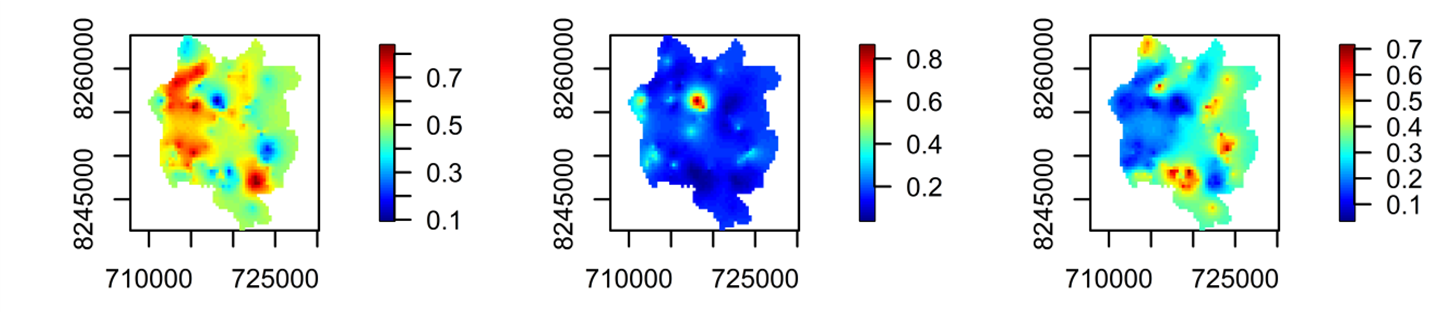
\includegraphics[scale=0.95]{Conditional probability - Multi-type.png}
    \end{center}
    \FigureCaption{Conditional probability that a point at each location is of a
    particular type: clade 0 (Left Panel), clade 2 (Middle Panel), grouped clades (Right Panel)} \label{fig:conditional-probability-multi-type}
\end{figure}

The left part of Figure \ref{fig:conditional-probability-multi-type} shows that typhoid fever cases caused by clade 0 sub-lineage of the multi-drug resistant H58 lineage of \textit{S. typhi} were dominant in the in the western side and south eastern side of Blantyre city. Specifically, clade 0 cases were dominant in the following areas: Chirimba, Kameza, Machinjiri, Nkolokoti-Kachere, Likhubula, Mbayani-Chemusa, Nancholi-Manase and Bangwe-Namiyango. The middle part shows that clade 2 was more dominant in Ndirande and Chilomoni. The grouped clades, that is clade 1, clade 3, clade 4, clade 5 and clade 6 were more dominant in the eastern part of Blantyre city. Specifically, the grouped clades were dominant in the following areas: Nancholi, Zingwangwa, Cholobwe-Misesa, Chigumula, Zingwangwa, Kachere, Mapanga, Machinjiri and Kameza.

Although Mbayani-Chemusa, Ndirande, Bangwe-Namiyango,  Nancholi-Manase and Nkolokoti-Kachere registered typhoid fever cases caused by multiple sub-lineages within the same location, the multi-type spatial analysis has shown that the sub-lineages were still competing and one of them was dominant than the others. For example, although Mbayani-Chemusa had high incidence rate of typhoid fever cases caused by all the three sub-lineages (clade 0, clade 2 and the grouped clades), clade 0 sub-lineage was more dominant than clade 2 and the grouped clades. Likewise, although Ndirande registered high incidence rate of typhoid fever cases caused by clade 0 and clade 2, conditional probability has shown that clade 2 was more dominant than clade 0. Similarly, Nancholi-Manase and Nkolokoti-Kachere registered typhoid fever cases caused by both clade 0 and the grouped clades. But conditional probability has shown that the grouped clades was more dominant than clade 0.

Figure \ref{fig:covariance-function-multi-type} shows the posterior covariance function for the Gaussian process of the multi-type spatial LGCP model. The figure shows that the posterior dependence between cells for all the sub-lineages is relatively bigger than the range for the spatio-temporal models in both time and space. The change can be attributed to the interactions between the sub-lineages.

\begin{figure}[H]
    \begin{center}
        \includegraphics[scale=0.8]{Posterior covariance function - Multi-type.png}
    \end{center}
    \FigureCaption{Posterior covariance function of the multi-type spatial model} \label{fig:covariance-function-multi-type}
\end{figure}
